\chapter{Release}

De software kan niet op een simpele manier gereleased worden aangezien deze complex is en uit meerdere onderdelen bestaat. Om te zorgen dat releases netjes gedocumenteerd en uitgerold worden is het releaseproces opgesteld. Hieronder is het proces kort beschreven.

\begin{enumerate}
	\item Branch van master met de naam "release-MAJOR.MINOR.PATCH"
	\item Voer unit tests uit op deze branch
	\item Voer integratietesten uit op deze branch
	\item Indien fouten opkomen zullen hotfixes worden uitgevoerd tot de testen niet meer falen
	\item Tag de release met de naam "release-MAJOR.MINOR.PATCH"
	\item Cherry-pick hotfixes naar de "master" branch
\end{enumerate}

Dit proces maakt gebruikt van het cactusmodel voor git, waarbij het werk zelf gebeurt in de master branch en de releases apart gezet worden. Hotfixes worden teruggezet in master.
\begin{figure}[h]
	\centering
	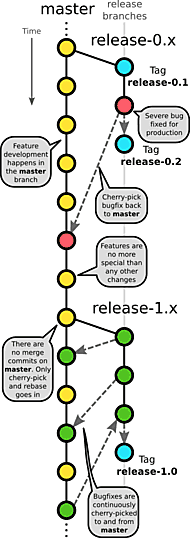
\includegraphics[height=7.7cm]{figures/cactus-model-100}	
	\caption{Een voorbeeld van het cactus-model}
	\label{fig:branch1}
\end{figure}
